\section{Related Work}
\label{sec:related_work}

\paragraph{Single-Intent Detection Datasets} 
We present datasets for single-intent detection, which serve as the foundation for more complex settings.
One of the classic resources in the field of intent detection is the ATIS dataset \citeplanguageresource{mansour2021atis}, which includes utterances about 26 airline-related intents.\footnote{Indeed, 8 of the original 26 intents in ATIS are multi-intent classes, which we exclude from our analysis.}
Meanwhile, the SNIPS dataset \citeplanguageresource{coucke2018snips} consists of utterances with 7 intents. 
These two datasets have extensions in MID settings, i.e., MixATIS and MixSNIPS \citeplanguageresource{qin-etal-2020-agif}.

Besides ATIS and SNIPS, there exist many other datasets for (single-)intent detection. 
We aim to expand upon these datasets by introducing them to the MID setting, similar to the cases of MixATIS and MixSNIPS.
One of the candidates within the scope of our study is Banking77 \citeplanguageresource{casanueva-etal-2020-efficient}, a dataset that comprises 13,083 customer service queries with 77 labeled intents specific to the banking domain.
Another target of our study is CLINC150 \citeplanguageresource{larson-etal-2019-evaluation}. 
This dataset encompasses 23,700 examples distributed across 150 intents within 10 domains, and offers additional distinct out-of-domain (OOD) instances.\footnote{For our purpose, we exclude data instances with the out-of-domain (OOD) intent, having a total of 150 intents.}

In summary, our work centers on four single-intent datasets---ATIS, SNIPS, Banking77, and CLINC 150---along with their extension into MID environments.\footnote{We leave exploration on other datasets, e.g., HWU64 \citeplanguageresource{liu2019benchmarking}, SLURP \citeplanguageresource{bastianelli-etal-2020-slurp}, and RedWood \citeplanguageresource{larson2022redwood}, as future work.}
In the following, we illustrate the current status and limitations of existing MID datasets. 

\begin{figure*}[t]
    \begin{center}
        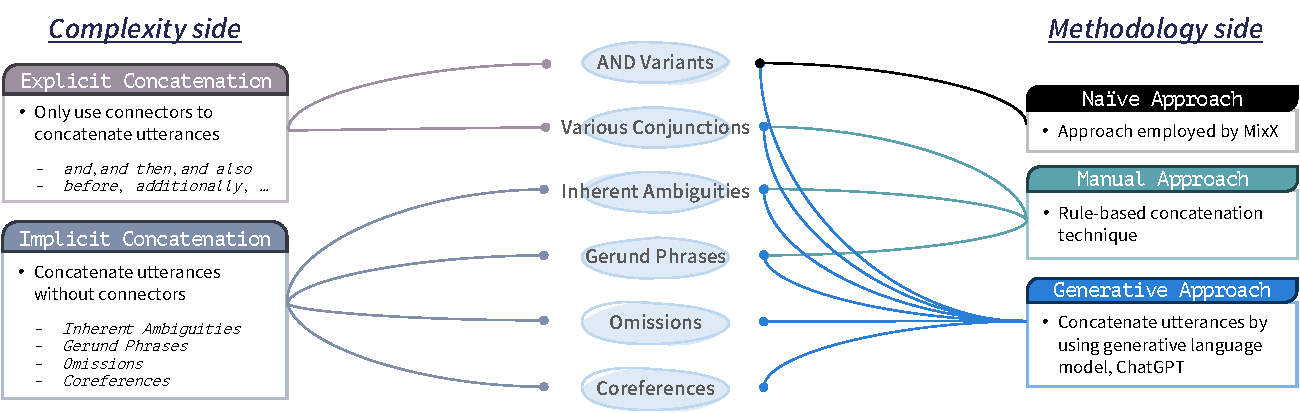
\includegraphics[scale=0.7]{images/Figure_2.pdf} 
        \caption{Illustration of the complexity (Left) and methodology (Right) aspects of concatenation. 
        Each approach triggers a distinct part of the possible variations (Middle) arising in the process of concatenation.}
        \label{fig:concat}
    \end{center}
\end{figure*}

\paragraph{Multi-Intent Detection Datasets} 
\citet{larson2022survey} indicate the scarcity of resources tailored for multi-intent detection.
Notably, MixATIS and MixSNIPS \citeplanguageresource{qin-etal-2020-agif} have played a pivotal role in supporting nearly every experiment in MID.
Since MixATIS and MixSNIPS were both proposed by the same group of researchers \citeplanguageresource{qin-etal-2020-agif}, they share common characteristics.
The datasets consist of utterances with up to three intents, and the distribution of inputs with different intents (1:2:3) is maintained at a ratio of 3:5:2.
Furthermore, they consistently utilize the term \texttt{`and'} (along with its variations) to merge multiple utterances into a unified one.
We also note that the \texttt{`,(comma)'} is used in the datasets exclusively when concatenating three utterances in a row.

These explicit patterns can provide strong cues for models. 
For example, a model might learn to identify the number of intents by either (1) counting the occurrences of the conjunction \texttt{`and'} or (2) recognizing the presence of a \texttt{`,(comma)'} indicating three intents.
If this hypothesis holds true, models trained on MixX may encounter notable performance drops when evaluated on datasets lacking or having fewer clues.
We thus intend to verify our conjecture by introducing a novel suite of datasets equipped with more diverse patterns.

Lastly, the recently introduced dataset named DialogUSR \citeplanguageresource{meng-etal-2022-dialogusr} stands out as a significant resource for MID research.
This dataset is characterized by its provision of pairs consisting of a multi-intent utterance and its corresponding single-intent sub-queries, all annotated by humans.
As a result, it enables models to learn the process of dissecting a multi-intent utterance and accurately extracting the resulting single-intent sub-queries.
However, its dependence on human annotations presents a clear drawback due to the associated costs. 
Furthermore, the dataset is built on the assumption that multi-intent utterances can be completely segmented, which may not hold true in real-world scenarios.